As mentioned in Chapter~\ref{ch:introduction}, swarm behaviors, are emergent behaviors that arise from the interactions of a number of animals in a group, whose individual behaviors tend to be relatively simple~\cite{Camazine2001}. To understand swarm behaviors, researchers in artificial intelligence and robotics devoted to mimicking the swarm behaviors such as foraging, aggregation and flocking observed in nature using simulated agents or physical robots. This approach is what we refer to as understanding from synthesis, and it has been shown to provide a deep insight to validate the models of swarm behaviors or generate new hypothesis~\cite{J.Halloy2007}. The design of the controllers for the agents and robots comply with some common principles. For example, the controllers are distributed, that is, there is no central control for the whole swarm. The structure of the controllers is relatively simple. Therefore, the models developed in distributed robotics could be used for validating our coevolutionary approach.

To validate our coevolutionary method, we present two case studies on canonical problems in distributed robotics: self-organized aggregation~\cite{Gauci2014_ijrr} and object clustering~\cite{Melvin2014_aamas}. In both swarm behaviors, individuals execute simple behavioral rules, but these lead to meaningful emergent behaviors on a global level. In this chapter, we only present the simulation results (a real world validation using a case study will be presented in Chapter~\ref{ch:swarm_physical_implementation}). We show that observing the individuals' motion is sufficient to guide the learning of these collective behaviors. 

This chapter is organized as follows. Sec.~\ref{sec:problem_formulation} describes the problem formulation. Sec.~\ref{sec:swarm_behaviors} describes the two swarm behaviors under investigation. Sec.~\ref{sec:simulation_platform} introduces the simulation platform. Sec.~\ref{sec:simulation_setup} details the experimental setups for learning the swarm behaviors. Sec.~\ref{sec:algorithm_implementation_swarm} details the implementation of the coevolutionary approach. Sec.~\ref{sec:results_simulation_swarm} presents the results obtained from the two case studies. Sec.~\ref{sec:summary_simulation_swarm} summaries the findings.

\section{Problem Formulation}\label{sec:problem_formulation}

The agents used in our case studies are embodied and move in a two-dimensional, continuous space. In both behaviors, each agent is equipped with one line-of-sight sensor that makes it able to distinguish between types of items in the environment (e.g., the background and other agents)~\cite{Gauci2014_ijrr}, \cite{Melvin2014_aamas}. In the case of object clustering, the objects to be clustered can also be distinguished by the agents. 
%
\begin{figure}[!t]
	\centering
	\includegraphics[width=3.5in]{e-puck_body.png}
	\caption{An e-puck robot fitted with a black `skirt' for visual distinction by other robots, and a top marker for motion tracking.}
	\label{fig:e-puck_body}
\end{figure}
%
The agents' embodiment is based on the e-puck~\cite{e-puck}, which is a miniature, differential-wheeled robot. Fig.~\ref{fig:e-puck_body} shows an e-puck robot used in the physical experiments which will be introduced in Chapter~\ref{ch:swarm_physical_implementation}.

The swarm behaviors investigated in this thesis use a reactive control architecture, in which the agents directly map their sensor states to motor actions and thus need no memory. This reactive control architecture can be found in many biological systems. For example, researchers have found that the complex auditory orientation behavior of female crickets is derived from simple reactive motor responses to specific sound pulses~\cite{Hedwig2004}. In social behaviors, ants simply follow the pheromone trails when foraging~\cite{Carroll1973}. 

In these two swarm behaviors, the motion of each agent depends on the state of the line-of-sight sensor ($I$). The controller is a mapping from each possible sensor state $I\in\{0,1,\cdots,n-1\}$ onto a pair of predefined velocities for the left and right wheels: $I  \rightarrow (v_{lI}, v_{rI})$. $v_{lI}, v_{rI} \in \left[-1,1\right]$ represent the normalized left and right wheel velocities, respectively, where $1$ ($-1$) corresponds to the wheel rotating forwards (backwards) with maximum velocity. The controller is simply a look-up table: given $n$ sensor states, any reactive behavior in this framework can be represented using $2n$ system parameters. In the rest of this thesis, we describe such controllers by writing the $2n$ parameters as a tuple in the following order:
\begin{equation}\label{controller:form}
\mathbf{p} = (v_{\ell 0}, v_{r0}, v_{\ell1}, v_{r1}, \cdots, v_{\ell (n-1)}, v_{r (n-1)}).
\end{equation}

The system identification task is to infer the parameters of the controllers in Eq~\eqref{controller:form} that govern the interaction between the agents. 
%
\section{Swarm Behaviors}\label{sec:swarm_behaviors}

In this section, we detail the behavioral rules of these two swarm behaviors. They both use the reactive control architecture in Sec.~\ref{sec:problem_formulation}.

\subsection{Aggregation Behavior}\label{sec:aggregation_behavior}

\captionsetup[subfigure]{labelformat=empty}  
\begin{figure}[!t]
	\centering
	\subfloat[initial configuration]{
		\includegraphics[width = 1.75 in]{snapshot_aggregation_initial.pdf}
	}
	\subfloat[after $60$ $\unit{s}$]{
		\includegraphics[width = 1.75 in]{snapshot_aggregation_60s.pdf}
	}\\
	\subfloat[after $180$ $\unit{s}$]{
		\includegraphics[width = 1.75 in]{snapshot_aggregation_180s.pdf}
	}
	\subfloat[after $300$ $\unit{s}$]{
		\includegraphics[width = 1.75 in]{snapshot_aggregation_300s.pdf}
	}
	\caption{Snapshots of the aggregation behavior of $50$ agents in simulation. }
	\label{fig:aggregation_snapshoot}
\end{figure}
%
In this behavior, the sensor is binary, that is, $n=2$. It gives a reading of $I=1$ if there is an agent in the line of sight, and $I=0$ otherwise. The agents are homogeneous: they all execute the same behavior. The environment is free of obstacles. The objective for the agents is to aggregate into a single cluster that is as compact as possible, as quickly as possible. Details of this behavior, including a validation with 40 physical e-puck robots, are reported in~\cite{Gauci2014_ijrr}. 

The `optimal' controller for aggregation was found by performing a grid search over the entire space of possible controllers (with finite resolution)~\cite{Gauci2014_ijrr}. In the form of Eq.~\eqref{controller:form}, the `optimal' controller's parameters are:
\begin{equation}\label{eq:aggregation_optimal_controller}
\mathbf{p} = \left(-0.7, -1.0, 1.0, -1.0\right). 
\end{equation}

When $I=0$, an agent moves backwards along a clockwise circular trajectory. When $I=1$, an agent rotates clockwise on the spot with maximum angular velocity. Note that rather counter-intuitively, an agent never moves forward, regardless of $I$. With this controller, an agent provably aggregates with another agent or a quasi-static cluster of agents~\cite{Gauci2014_ijrr}. Fig.~\ref{fig:aggregation_snapshoot} shows snapshots from a simulation trial.

\subsection{Object Clustering Behavior}
This behavior uses $n=3$ sensor states: $I=0$ if the sensor is pointing at nothing (or the wall of the environment, if the latter is bounded), $I=1$ if the sensor is pointing at an object, and $I=2$ if it is pointing at another agent. The aim of the agents is to arrange the objects into a single cluster as fast as possible. Details of this behavior, including a validation using 5 physical e-puck robots and 20 cylindrical objects, are presented in~\cite{Melvin2014_aamas}.

In the form of Eq.~\eqref{controller:form}, the `optimal' controller's parameters, found using an evolutionary algorithm~\cite{Melvin2014_aamas}, are:
\begin{equation}\label{eq:clustering_optimal_controller}
\mathbf{p} = \left( 0.5, 1.0, 1.0, 0.5, 0.1, 0.5 \right).
\end{equation} 

\captionsetup[subfigure]{labelformat=empty}  
\begin{figure}[!t]
	\centering
	\subfloat[initial configuration]
	{
		\includegraphics[width = 1.75 in]{snapshot_clustering_initial.pdf}
	}
	\subfloat[after $20$ $\unit{s}$]{
		\includegraphics[width = 1.75 in]{snapshot_clustering_20s.pdf}
	}\\
	\subfloat[after $40$ $\unit{s}$]{
		\includegraphics[width = 1.75 in]{snapshot_clustering_40s.pdf}
	}
	\subfloat[after $60$ $\unit{s}$]{
		\includegraphics[width = 1.75 in]{snapshot_clustering_60s.pdf}
	}\\
	\caption{Snapshots of the object clustering behavior in simulation. There are $5$ agents (blue) and 10 objects (green).}
	\label{fig:clustering_snapshoot}
\end{figure}

When $I=0$ and $I=2$, the agent moves forward along an anti-clockwise circular trajectory, but with different linear and angular speeds. When $I=1$, it moves forward along a clockwise circular trajectory. Fig.~\ref{fig:clustering_snapshoot} shows snapshots from a simulation trial.

\section{Simulation Platform}\label{sec:simulation_platform}

We use the open-source Enki library~\cite{Enki}, which has a built-in model of the e-puck. This is represented as a disk\footnote{Enki does not model height as it is a two-dimensional simulator. The physical e-puck's height is around $\unit[7.0]{cm}$.} of diameter $\unit[7.4]{cm}$ and mass $\unit[150]{g}$. The inter-wheel distance is modeled as $\unit[5.1]{cm}$, and the speed of each wheel can be set independently. Enki induces some noise on the wheel speeds by multiplying the set value by a number in the range $(0.95, 1.05)$ chosen randomly with uniform distribution. The maximum speed of the e-puck is $\unit[12.8]{\textrm{cm/s}}$, forward or backward. Although Enki models the e-puck's real sensors, we choose to implement the line-of-sight sensor independently, for the sake of accuracy (in the physical experiments, this sensor is realized using the e-puck's camera; see Chapter~\ref{ch:swarm_physical_implementation}). The line-of-sight sensor is simulated by casting a ray from the e-puck's front and checks the first item with which it intersects (if any). The range of this sensor is unlimited in simulation. In the object clustering behavior, we model objects as disks of diameter $\unit[10]{cm}$ with mass $\unit[35]{g}$ and a coefficient of static friction with the ground of $0.58$, which makes it movable by a single e-puck.

Enki models the kinematics and dynamics of all items in the environment (i.e., robots and objects), and also handles the physics (e.g., collisions). In all simulations, we use an unbounded environment. The physics and robots' control cycle are updated every $\unit[0.01]{s}$ and $\unit[0.1]{s}$, respectively.

\section{Experimental Setups}\label{sec:simulation_setup}
In the aggregation setup, we used $11$ individuals---$10$ agents and $1$ replica that executes a model. The initial positions of individuals were generated randomly in a square region of sides $\unit[331.66]{cm}$, following a uniform distribution (average area per individual = $\unit[10000]{cm^2}$). 

In the object clustering setup, we used $5$ individuals---$4$ agents and $1$ replica that executes a model---and $10$ cylindrical objects. The initial positions of individuals and objects were generated randomly in a square region of sides $\unit[100]{cm}$, following a uniform distribution (average area per object = $\unit[1000]{cm^2}$). In both setups, each individual's starting orientation was chosen randomly in $[-\pi,\pi]$ with uniform distribution.

%For both case studies, the model and classifier populations each consisted of $100$ solutions. In each trial, classifiers observed individuals for $\unit[10]{s}$ at $\unit[0.1]{s}$ intervals ($100$ time steps).

\section{Coevolutionary System Identification without Metrics}\label{sec:algorithm_implementation_swarm}

The coevolutionary algorithm in our approach comprises two populations, one of models, and one of classifiers, which coevolve competitively. The fitness of the classifiers depends solely on their ability to distinguish the behavior of the model from the behavior of the agents. The fitness of the models depends solely on their ability to mislead the classifiers into making the wrong judgment, that is, classifying them as an agent.

\subsection{Model Structure} 

The model is to be executed on a replica, which resembles the agent under investigation in terms of appearance\footnote{As shown in Chapter~\ref{ch:literature_review}, the appearance of the replica might be `similar'  to the agents from their visual perspective but it is not necessary to be similar in terms of human eye.} and behavioral abilities. In particular, we assume that the replica also has a line-of-sight sensor\footnote{In Sec.~\ref{sec:evolving_control_and_morphology}, we show that this assumption can be relieved by evolving the angle of view of the sensor.}. The task is thus to estimate the parameters of the aggregation and object clustering controllers (shown in Eqs.~\eqref{eq:aggregation_optimal_controller} and~\eqref{eq:clustering_optimal_controller}), respectively. This makes it possible for us to objectively measure the quality of the models obtained and thus the performance of our coevolutionary approach (as discussed in the results section). Note that the classifiers do not have any prior knowledge about the individuals under investigation. To make the evolution more challenging, the search space for the algorithm in simulation is unbounded. That is, the model parameters are unconstrained, and the replica can move with arbitrary speed. 

\begin{figure}[!t]
	\centering
	\includegraphics[width=3.0 in]{Neural_Network_CF_Swarm.pdf}
	\caption{The structure of the classifiers is a recurrent Elman neural 
    network with two inputs (agent linear speed, $v$ and angular speed, $w$), five hidden neurons, and one output neuron ($O$). $O$ is used for making a judgment. Two bias neurons (which are not shown) with a constant input of 1.0 are connected to each neuron of the hidden and output layers. See text for details.}
	\label{fig:neural_network_cf_swarm}
\end{figure}

\subsection{Classifier Structure}

The structure of the classifier is shown in Fig.~\ref{fig:neural_network_cf_swarm}. It is a recurrent Elman neural network~\cite{Elman1990} with two inputs, five hidden neurons and one output neuron. Each neuron of the hidden and output layers has a bias. Note that the number of hidden neurons was chosen arbitrarily and we did not attempt to optimize the number required. The network has a total of $46$ parameters, which all assume values in $\mathbb{R}$. The activation function used in the hidden and the output neurons is the logistic sigmoid function, which has the range $\left(0,1\right)$ and is defined as: 
%
\begin{equation}\label{equ:logistic_sigmoid}
\textrm{sig}\,x = \frac{1}{1+e^{-x}}\quad\forall x \in \mathbb{R}.
\end{equation}
%
The two inputs to the network are the linear speed ($v$) and angular speed ($\omega$) of the individual. They are obtained by tracking the positions and orientations of individuals in real time. In simulation, the tracking is noise-free. We define the linear speed to be positive when the angle between the individual's orientation and its direction of motion is smaller than $\unit[\pi \small/ 2]{rad}$ (i.e., the individual is moving forward), and negative otherwise. 

The classifier observes the motion of each individual over a set period of time. The initial configuration\footnote{Throughout this paper, `initial configuration' refers to initial positions and orientations (of the individuals) or initial positions (of the objects).} of the individuals are randomly generated in each trial. After the end of the trial, all classifiers are provided with the motion data of all individuals. For each classifier, after being fed all the observed data of an individual from a trial, the final value of its output neuron (which is defined as $O$), is used to make a judgment: the classifier decides `model' if $O<0.5$, and `agent' if $O\geq0.5$. The classifier's memory is reset after each judgment.

\subsection{Optimization Algorithm}\label{sec:optimization_algorithm_swarm}
The optimization algorithm used is based on a ($\mu+\lambda$) evolution strategy with self-adaptive mutation strengths~\cite{Beyer2001, Beyer2002, Eiben2003}, and can be thought of consisting of two sub-algorithms: one for the model population, and another for the classifier population. Both populations are treated identically. They do not interact with each other except for the fitness calculation step (described later in Sec.~\ref{sec:fitness_calculation_swarm}). In each sub-algorithm, the value of $\mu$ and $\lambda$ is equal, which is half of the population size. 

For both case studies, the model and classifier populations each consisted of $100$ solutions. In each trial, classifiers observed individuals for $\unit[10]{s}$ at $\unit[0.1]{s}$ intervals ($100$ time steps). In the following, we detail the implementation of the evolutionary algorithm.

In this algorithm, an individual is a 2-tuple,
$\mathbf{a}=\left(\mathbf{x},\boldsymbol{\sigma}\right)$, where $\mathbf{x\in\mathbb{R}}^n$ represents objective parameters, and $\boldsymbol{\sigma}\in \left(0,\infty\right)^n$
represents mutation strengths. The $i$-th mutation strength in $\boldsymbol{\sigma}$ corresponds to the $i$-th element in $\mathbf{x}$. For the model sub-algorithm, $n=4$ (for aggregation) or $6$ (object clustering), for the classifier sub-algorithm, $n=46$.

Each generation $g$ comprises a population of $\mu=50$ individuals:
\begin{displaymath}
\mathcal{P}^{\left(g\right)} = \left\{\mathbf{a}_1^{\left(g\right)}, 
\mathbf{a}_2^{\left(g\right)},\dots,\mathbf{a}_{\mu}^{\left(g\right)}\right\}.
\end{displaymath}
In the population of the first generation, $\mathcal{P}^{\left(0\right)}$, all the objective parameters are initialized to $0.0$ and all the mutation strengths are initialized to $1.0$. Thereafter, in every generation $g$, the $\mu$ parent individuals are first used to create $\lambda=50$ offspring individuals by recombination. For the generation of each recombined individual $\mathbf{a}^{\prime\left(g\right)}_k$, $k\in\left\{1,2,\dots,\lambda\right\}$, two individuals are chosen randomly, with replacement, from the parent population: $\mathbf{a}^{\left(g\right)}_{\chi}$ and $\mathbf{a}^{\left(g\right)}_{\psi}$, where $\chi,\psi\in\left\{1,2,\dots,\mu\right\}$. The intermediate population,  $\mathcal{P}^{\prime \left(g\right)}$, is produced using discrete and intermediate recombination, which generates the objective parameters and the mutation strengths of the recombined individual, respectively:
\begin{eqnarray}
x_{k,i}^{\prime\left(g\right)} & = & x_{\chi,i}^{\left(g\right)} \textrm{\quad OR\quad} x_{\psi,i}^{\left(g\right)},\label{eq:x_recomb}\\
\sigma_{k,i}^{\prime\left(g\right)} & = & \left(\sigma_{\chi,i}^{\left(g\right)} + \sigma_{\psi,i}^{\left(g\right)}\right)/2,
\end{eqnarray}
where $i\in\left\{1,2,\dots,n\right\}$ is indexing the elements within the vectors and, in Eq.~\ref{eq:x_recomb}, the selection is performed randomly and with equal probability.

Each of the $\lambda$ recombined individuals is then mutated in order to obtain the final offspring population, $\mathcal{P}^{\prime\prime \left(g\right)}$. This is done according to:
\begin{eqnarray}
\sigma_{k,i}^{\prime\prime \left(g\right)} & = & 
\sigma_{k,i}^{\prime\left(g\right)} \exp\left(\tau^{\prime} \mathcal{N}_{k}\left(0,1\right)
+ \tau \mathcal{N}_{k,i}\left(0,1\right) \right), \label{eq:sigma_mutation}\\
x_{k,i}^{\prime\prime \left(g\right)} & 
= & x_{k,i}^{\prime\left(g\right)} + \sigma_{k,i}^{\prime\prime \left(g\right)}
\mathcal{N}_{k,i} \left(0,1\right), \label{eq:x_mutation}
\end{eqnarray}
for all $\left\{k,i\right\}$, where $k\in\left\{1,2,\dots,\lambda\right\}$ is indexing the individuals within the population and $i\in\left\{1,2,\dots,n\right\}$ is indexing the elements within the vectors. Eq.~\ref{eq:sigma_mutation} generates the perturbed mutation strength from the original one according to a log-normal distribution. Eq.~\ref{eq:x_mutation} mutates the objective parameter according to a normal distribution having the perturbed mutation strength as its deviation. In Eq.~\ref{eq:sigma_mutation}, $\mathcal{N}_{k}\left(0,1\right)$ and $\mathcal{N}_{k,i} \left(0,1\right)$ are both random numbers generated from a standard normal distribution; however, the former is generated once for each individual (i.e. for each value of $k$), while the latter is generated separately for each element within each individual (i.e. for each combination of $k$ and $i$). The parameters $\tau^{\prime}$ and $\tau$ determine the learning rates of the mutation strengths, and are set as $\tau^{\prime} = 1/2\sqrt{2n}$, $\tau = 1/2\sqrt{2\sqrt{n}}$ (similar to~\citep{Yao1999}).

Once the offspring population has been generated, the $\mu$ individuals with the highest fitness (see Sec.~\ref{sec:fitness_calculation_swarm}) from the combined population, $\mathcal{P}^{\left(g\right)}\cup \mathcal{P}^{\prime\prime\left(g\right)}$ (which contains $\mu+\lambda$ individuals), are selected as the parents to form the population of the next generation, $\mathcal{P}^{\left(g+1\right)}$. Individuals with an equal fitness have an equal chance of being selected.

\subsection{Fitness Calculation}\label{sec:fitness_calculation_swarm}
We will describe the fitness calculation process for the general case (i.e., without using specific parameter values). Note that we use different parameter settings in our simulation and physical (Chapter~\ref{ch:swarm_physical_implementation}) experiments.

Let the population sizes for the models and classifiers in the coevolution be $M$ and $N$, respectively. Let $m$ (factor of $M$) be the number of models to be executed on the replica(s), and $n$ be the number of agents in each trial. We only conduct one trial for each model. Therefore, in each generation, there are $\frac{M}{m}$ trials to be performed.

The fitness of a model in each generation is obtained by evaluating it with each of the $N$ classifiers in the competing population based on the model's observed motion in a trial. For every classifier that wrongly judges the model as an agent, the model's fitness increases by $1$. After all evaluations, the model's fitness takes a value in $\left\{0, 1, 2, \dots, N \right\}$. This value is then normalized to $[0, 1]$.

The fitness of each classifier in a trial is obtained by using it to evaluate $m$ models and $n$ agents. For each correct judgment of the model, the classifier's fitness for the models, $f_1$, increases by $\frac{1}{2m}$; for each correct judgment of the agent, the classifier's fitness for the agents, $f_2$, increases by $\frac{1}{2n}$. Therefore, the fitness of each classifier in a trial, $f = f_1 + f_2$, is in the range $[0, 1]$. This evaluation is performed $\frac{M}{m}$ times in each generation, and the fitness value of each classifier in that generation is then normalized to $[0, 1]$.
%Fitness values are to be optimized. is in the set $\left\{0, \frac{1}{2m}, \frac{1}{2n}, \frac{1}{2m} + \frac{1}{2n}, \dots, 1 \right\}$

\section{Results}\label{sec:results_simulation_swarm}

\subsection{Analysis of Evolved Models}\label{sec:analysis_evolved_models_swarm_simulation}

\begin{figure}[!t]%htbp
	\centering
		\subfloat[(a) Aggregation \label{fig:model_parameters_box_aggregation}]{%
			\includegraphics[width=3.5 in]{model_parameters_box_aggregation.pdf}
		}\\
		\subfloat[(b) Object Clustering\label{fig:model_parameters_box_clustering}]{%
			\includegraphics[width=3.5 in]{model_parameters_box_clustering.pdf}
		}
		\caption{Parameters of the evolved models with the highest subjective fitness in the $1000^\textrm{th}$ generation in the coevolutions for (a) the aggregation behavior and (b) the object clustering behavior. Each box corresponds to 30 coevolution runs in simulation. The dotted black lines correspond to the values of the parameters that the system is expected to learn (i.e., those of the agent).\label{fig:model_parameters_box}}
\end{figure}

\begin{figure}[!t]
	\centering
		\subfloat[(a) Aggregation \label{fig:model_validation_aggregation_simulation}]{%
			\includegraphics[width=3.5 in]{model_validation_aggregation_simulation.pdf}
		}\\
		\subfloat[(b) Object Clustering\label{fig:model_validation_clustering_simulation}]{%
			\includegraphics[width=3.5 in]{model_validation_clustering_simulation.pdf}
		}
		\caption{(a) Dispersion (after $\unit[400]{s}$) of $50$ agents all executing the real aggregation controller (red box) and each of the evolved models (blue boxes) in the $1000^\mathrm{th}$ generation. (b) Dispersion (after $\unit[400]{s}$) of $50$ objects in a swarm of $25$ agents all executing the real object clustering controller (red box) and each of the evolved models (blue boxes). In both (a) and (b), boxes show distributions over $30$ trials. The dotted black lines indicate the minimum dispersion that $50$ agents/objects can possible achieve~\cite{Graham1990}. See Sec.~\ref{sec:analysis_evolved_models} for details.\label{fig:model_validation_simulation}}
\end{figure}

We performed 30 coevolution runs for each setup. Each run lasted 1000 generations. Fig.~\ref{fig:model_parameters_box} shows a box plot\footnote{The box plots presented here are all as follows. The line inside the box represents the median of the data. The edges of the box represent the lower and the upper quartiles ($25^\mathrm{th}$ and $75^\mathrm{th}$ percentiles) of the data, whereas the whiskers represent the lowest and the highest data points that are within $1.5$ times the inter-quartile range from the lower and the upper quartiles, respectively. Circles represent outliers.\label{fn:boxplot}} with the parameters of the evolved models with the highest subjective fitness\footnote{Since the fitness of the models depends solely on the judgment of the classifiers during the coevolutionary process, it is commonly referred to as \textit{subjective}. In the rest of this thesis, unless otherwise stated, `evolved model' refers to the model with the highest subjective fitness in a generation.} in the final generation. The system identified the parameters of these two behaviors with good accuracy (dotted black lines represent the parameters of the observed swarming agents). In the case of aggregation, the means (standard deviations) of the AEs\footnote{Given an evolved controller $\mathbf{x}$ and a real controller $\mathbf{p}$, where $\mathbf{x},\mathbf{p}\in[-1,1]^{2n}$, we define the absolute error (AE) in a particular parameter $i\in\{1,2,\dots,2n\}$ as: $|x_i-p_i|$. We define the mean absolute error (MAE) over all parameters as: $\frac{1}{2n}\sum_{i=1}^{2n} |x_i-p_i|$. Throughout the main text, we exclusively use the acronyms AE and MAE. Therefore ``mean AE'' is not to be confused with MAE; rather, it refers to the mean AE in one parameter over a number of coevolution runs.} in the parameters (from left to right in Fig.~\subref*{fig:model_parameters_box_aggregation}) were: $0.01$ ($0.01$), $0.01$ ($0.01$), $0.07$ ($0.07$) and $0.06$ ($0.04$). In the case of object clustering, these values were: $0.03$ ($0.03$), $0.04$ ($0.03$), $0.02$ ($0.02$), $0.03$ ($0.03$), $0.08$ ($0.13$) and $0.08$ ($0.09$).

Although the evolved models approximate the agents well in terms of parameters, it has often been observed in swarm systems that small changes in individual agent behaviors can lead to vastly different emergent behaviors, especially with large numbers of agents~\cite{Paul2010, Luca2014}. For this reason, we evaluated the quality of the emergent behaviors that the models give rise to. In the case of aggregation, a good measure of the emergent behavior is the dispersion of the swarm after some elapsed time as defined in~\cite{Gauci2014_ijrr}\footnote{The measure of dispersion is based on the robots'/objects' distances from their centroid. For a complete definition, see Eq. (5) of \cite{Gauci2014_ijrr} and Eq. (2) of~\cite{Melvin2014_aamas}.}. For each of the $30$ models (see Fig.~\subref*{fig:model_parameters_box_aggregation}), we performed $30$ trials with $50$ agents each executing the model. For comparison, we also performed $30$ trials using the real controller (see Eq.~\eqref{eq:aggregation_optimal_controller}). The set of initial configurations was the same for all models and the real controller. Fig~\subref*{fig:model_validation_aggregation_simulation} shows the dispersion for the models and real controller after $\unit[400]{s}$. All models led to aggregation. We performed a statistical test\footnote{Throughout this thesis, unless otherwise stated, the statistical test used is a two-sided Mann-Whitney test with a $5\%$ significance level.} on the final dispersion of the agents between the real controller and each model. There was no statistically significant difference in $26$ out of $30$ cases without Bonferroni correction ($30$ out of $30$ cases with Bonferroni correction). 

In the case of object clustering, we use the dispersion of the objects after some elapsed time as a measure of the emergent behavior. With the real controller (see Eq.~\eqref{eq:clustering_optimal_controller}) and each of the models (see Fig.~\subref*{fig:model_parameters_box_clustering}), we performed $30$ trials with $25$ agents and $50$ objects. The results are shown in Fig.~\subref*{fig:model_validation_clustering_simulation}. In a statistical test on the final dispersion of the agents between the real controller and each model, there was no statistically significant difference in $24$ out of $30$ cases without Bonferroni correction ($26$ out of $30$ cases with Bonferroni correction).

\begin{figure}[!t]%
	\centering
		\subfloat[(a) Aggregation \label{fig:model_parameters_convergence_aggregation}]{%
			\includegraphics[width=3.5 in]{model_parameters_convergence_aggregation.pdf}
		}\\
		\subfloat[(b) Object Clustering\label{fig:model_parameters_convergence_clustering}]{%
			\includegraphics[width=3.5 in]{model_parameters_convergence_clustering.pdf}
		}
		\caption{Evolutionary process of the evolved model parameters for (a) the aggregation behavior and (b) the object clustering behavior. Curves represent median values across 30 coevolution runs. Dotted black lines indicate true values. \label{fig:model_parameters_convergence}}
\end{figure}

\subsection{Coevolutionary Dynamics}\label{sec:coevolutionary_dynamics_simulation_swarm_simulation}

We also investigated the evolutionary process of the model parameters. Fig.~\ref{fig:model_parameters_convergence} shows the convergence of the model parameters over generations. In the aggregation behavior, the parameters corresponding to $I=0$ were learned first. After about $50$ generations, both $v_{\ell0}$ and $v_{r0}$ closely approximated their true values ($-0.7$ and $-1.0$) shown in Fig.~\subref*{fig:model_parameters_box_aggregation}. For $I=1$, it took about $200$ generations for both $v_{l1}$ and $v_{r1}$ to converge. A likely reason for this effect is that an agent spends a larger percentage of its time seeing nothing ($I=0$) than other agents ($I=1$)---simulations revealed these percentages to be $8.8\%$ and $91.2\%$, respectively (mean values over 100 trials). 

In the object clustering behavior, the parameters corresponding to $I=0$ and $I=1$ were learned faster than the other two parameters corresponding to $I=2$, as shown in the Fig.~\subref*{fig:model_parameters_convergence_clustering}. After about $200$ generations, $v_{\ell0}$, $v_{r0}$, $v_{l1}$ and $v_{r1}$ started to converge; however it took about $400$ generations for $v_{l2}$ and $v_{r2}$ to approximate their true values. This is likely because an agent spends the most percentage of its time seeing nothing ($I=0$), followed by objects ($I=1$) and other agents ($I=2$)---simulations revealed these percentages to be $53.2\%$, $34.2\%$ and $12.6\%$ , respectively (mean values over 100 trials).

\begin{figure}[!t]%
	\centering
		\subfloat[(a) Aggregation \label{fig:fitness_curve_aggregation_simulation}]{%
			\includegraphics[width=3.5 in]{fitness_curve_aggregation_simulation.pdf}
		}\\
		\subfloat[(b) Clustering Objects\label{fig:fitness_curve_clustering_simulation}]{%
			\includegraphics[width=3.5 in]{fitness_curve_clustering_simulation.pdf}
		}
		\caption{This plot shows the subjective fitness of the classifiers and
		the models for (a) the aggregation behavior and (b) the clustering objects behavior.
		The curves show the median value across 30 coevolution runs.\label{fig:fitness_dynamics_simulation}}
\end{figure}

In order to analyze how the classifiers and the models interact with each other during the course of the coevolution, we investigate the dynamics of the subjective fitness of the classifiers and the models as shown in Fig.~\ref{fig:fitness_dynamics_simulation}. 

In the aggregation behavior, at the beginning, the fitness of the classifiers is 0.5 as they output 1 for all the agents and models, which means the classifiers make uninformed decisions\footnote{Note that in the implementation of the coevolutionary algorithm, the parameters of the models and classifiers are initialized to 0, which means all the classifiers are identical at the $1^{\mathrm{st}}$ generation.}. Therefore, the fitness of the models starts from 1.0, as all the classifiers judge them as the agent. Then, the average fitness of the classifiers quickly increases, corresponding to the decline of the average fitness of the models. As the models learn to adapt, the average fitness of the classifiers only increases slightly until about the $50^{\mathrm{th}}$ generation. After that, the average fitness of the models starts to increase. However, the best fitness of the classifiers is still higher than that of the models. The best fitness of the models surpasses that of the classifiers after about the $120^{\mathrm{th}}$ generation; at this point, the fitness of the `best' model is around $0.7$. This means that the `best' model is able to mislead $70\%$ of the classifiers into judging it as the agent. From the $200^{\mathrm{th}}$ generation onwards, the fitness of the classifiers and models remains ``balanced'' until the last generation. 

The coevolutionary dynamics of the object clustering behavior is similar. Compared with the dynamics of the aggregation behavior, it takes more generations for the fitness of the models to surpass that of the classifiers. This could be explained by the higher number of parameters and the higher complexity of the behavior to be evolved in the object clustering behavior.
\begin{figure}[!t]
	\centering
	\includegraphics[width=3.5in]{all_generation_judgment_accuracy.pdf}
	\caption{The average performance of the best classifiers and the classifier systems selected using a grid evaluation (see Eq.~\eqref{classifier:metric}) and the available (recorded) data over generations in $30$ coevolution runs. The error bar shows standard deviation.}
	\label{fig:all_generation_judgment_accuracy}
\end{figure}

\begin{figure}[!t]%
	\centering
		\subfloat[(a) decision-making process\label{fig:classifier_output_sequence}]{%
			\includegraphics[width=3.0 in]{classifier_output_sequence.pdf}
		}\\
		\subfloat[(b) activation of hidden neurons\label{fig:classifier_output_hidden_neurons}]{%
			\includegraphics[width=3.0 in]{classifier_output_hidden_neurons.pdf}
		}
		\caption{This plot shows the (a) decision-making process and (b) the corresponding activation value of the $5$ hidden neurons of a classifier for three random-chosen agents and the replica that executes a very good model in a trial. Hidden neurons are labeled as $\textrm{h}1$, $\textrm{h}2$, $\textrm{h}3$, $\textrm{h}4$, and $\textrm{h}5$.}
		\label{fig:classifier_output}
\end{figure}

\subsection{Analysis of Evolved Classifiers}\label{sec:analysis_evolved_classifiers_swarm_simulation}

The main product of the coevolutionary algorithm is the model, discussed in the previous section. However, the evolved classifiers can also be considered as a useful byproduct; for instance to detect abnormal agents in a swarm. We will now analyze the performance of the evolved classifiers, and discuss how to construct a robust classifier system---comprising multiple classifiers in tandem---from a coevolution run. For conciseness, we consider only the aggregation case study.

In practice, it would be ideal if classifiers could be post-evaluated and selected based on motion data that is already available from the trials performed in a coevolution run. To analyze whether this approach is feasible, we compare it against one that uses a more objective measure of classifier performance. Roughly speaking, this measure evaluates for what proportion of the entire model space a classifier is able to make correct judgments when a model is mixed into a group of agents.

We now present a formal description of this measure. We consider models uniformly distributed across the entire parameter space of the agents: $[-1,1]^4$. To keep the analysis of classifiers within a reasonable computation time, we discretize this space using $11$ settings per parameter, to obtain: $\mathcal{X} = \{-1.0, -0.8, ..., 0.8, 1.0\}^4$. This discretized space is a grid consisting of $|\mathcal{X}|=11^4=14641$ points (i.e., models). The classifier's performance on each model is computed as follows. The model is executed by a replica mixed into a group of $10$ agents (as in the coevolution runs). $10$ trials are performed using a set of initial configurations common to all classifiers. In each trial, the fitnesses of the classifier for the models ($f_1$) and agents ($f_2$) are calculated according to Sec.~\ref{sec:fitness_calculation_swarm}. Note that as we use $m=1$ replica and $n=10$ agents, $f_1\in\{0,0.5\}$, while $f_2\in\{0,0.05,\dots,0.5\}$. After the $10$ trials, the average fitnesses $\bar{f}_1$ and $\bar{f}_2$ are computed. The classifier's overall performance is computed as the average over all models and agents (higher values represent better classifiers):
%Based on these $10$ trials, the classifier gets two scores: $f_1$ and $f_2$. For each correctly identified model ($1$ in each trial), $f_1$ increases by $0.1$. For each correctly identified agent ($10$ in each of the $10$ trials), $f_2$ increases by $0.01$. Therefore, $f_1$ and $f_2$ each receive a value in $[0, 1]$. 
\begin{equation}\label{classifier:metric}
F_{\textrm{grid}}=\frac{1}{|\mathcal{X}|} \sum_{\mathbf{x}\in \mathcal{X}} \bar{f}_1(\mathbf{x}) + \bar{f}_2(\mathbf{x}).
\end{equation}
%
%
When assessing a classifier's performance using motion data from the coevolution run, this is done in a similar way as Eq.~\eqref{classifier:metric}. The classifier is evaluated using data from every trial that has been performed. For each trial, $f_1$ and $f_2$ are calculated, and the overall performance is computed as the average of $f_1 + f_2$. We term this measure $F_\textrm{data}$.

\subsubsection{Using a Single Classifier}
In each generation of every coevolution run, we performed two orderings of the classifiers in that generation, using $F_\textrm{grid}$ and $F_{\textrm{data}}$. Note that when evaluating $F_\textrm{data}$, only trials performed until that generation were used (i.e., as if the coevolution had been terminated at that generation). The best classifier according to each ordering was selected. We term these the ``grid-best-classifier'' and ``data-best-classifier''. For a fair and more objective comparison of these two classifiers, the performance of the data-best-classifier was re-evaluated using $F_\textrm{grid}$. The results (red and blue) are shown in Fig.~\ref{fig:all_generation_judgment_accuracy}.

At the start of the coevolution, the performance of the grid-best-classifier (red) increases rapidly with progressing generations; a high performance of $0.9$ (on average) is reached after only $10$ generations. The performance then continues improving slowly, reaching more or less a plateau by generation $100$.
The performance of the data-best-classifier (blue) also increases rapidly in the first $10$ generations, but is slightly below that of the grid-best-classifier. After this point, however, a strikingly different trend is observed. The performance starts \emph{decaying}, dropping to around $0.65$ by the $1000^\textrm{th}$ generation.

At first sight, it is counter-intuitive that selecting the data-best-classifier with more data leads to worse results. This phenomenon, however, can be explained when considering the model population. We have shown in the previous section (see especially Fig.~\subref*{fig:model_parameters_convergence_aggregation}) that the models converge rapidly at the beginning of the coevolution. As a result, when classifiers are evaluated in later generations, many of the trials considered include models very similar to each other. The selected classifiers thus become overspecialized to a small set of models: the ones dominating the later generations. Consequently, these classifiers have a low performance when evaluated across the entire model space (i.e., using $F_\textrm{grid}$).

Fig.~\ref{fig:classifier_output} shows the decision-making process and the corresponding activation value of the $5$ hidden neurons of the best classifier in the last generation of a coevolution run for $3$ randomly-chosen agents and the replica in a trial. The model executed on the replica has a parameter set of $(-0.7, -1.0, 1.0, -0.9)$, which is very near to that of the agent in Eq.\eqref{eq:aggregation_optimal_controller}. As we can see in Fig.~\subref*{fig:classifier_output_sequence}, for the agents, the classifier outputs $0$ at the beginning, and then starts to output $1$ after certain time steps, which means it needs some time to make the correct judgment. Note that for some time steps after it starts to output $1$, it still outputs $0$, but this happens only occasionally. For the model, it always outputs $0$.  This phenomenon can be explained by the activation value of the hidden neurons of the classifier in the following paragraph.

The classifier's activation value of the hidden neurons (labeled as $\textrm{h}1$, $\textrm{h}2$, $\textrm{h}3$, $\textrm{h}4$, and $\textrm{h}5$) shown in Fig.~\subref*{fig:classifier_output_hidden_neurons} reveals its internal processing for the motion of different individuals\footnote{Note that the activation of hidden neurons may not be the same for all the classifiers due to the symmetry of neural networks, but the dynamics of each hidden neuron is similar.}. It seems that the decision-making (``sudden jump'' in Fig.~\subref*{fig:classifier_output_sequence}) of the classifier is most likely related with the variation of $\textrm{h}3$ and $\textrm{h}4$. Take the agents for example, at the beginning, $\textrm{h}3$ has a very low value (which is almost $0$) and then after certain time steps it starts to increase. The variation tendency of $\textrm{h}4$ is opposite.  Every time the classifier's judgment starts to jump from $0$ to $1$, the value of $\textrm{h}3$ starts to surpass that of $\textrm{h}4$. $\textrm{h}1$, $\textrm{h}2$ and $\textrm{h}5$ are almost not activated during the whole period, although sometimes the activation of $\textrm{h}2$ influences the judgment of the classifier. For instance, there are two peaks at about $50^\textrm{th}$ and $80^\textrm{th}$ time step in $\textrm{h}2$ for agent two and three, which corresponds to a wrong judgment of the classifier (that is, it outputs $0$) at the same point. For the model, all the hidden neurons are almost not activated.

\subsubsection{Using a Classifier System}
The results of the previous section have shown that using a single classifier selected using $F_{\textrm{data}}$ is not a feasible solution (although there may be reasonably good classifiers in early generations, it is not known when the decay in performance begins).

To address this problem, we propose the use of a classifier system, that is, a number of classifiers working in tandem to judge a given candidate. We choose the best $10$ classifiers\footnote{
%
There is no guarantee that the individually best few classifiers will form the best \emph{system} when working in tandem. In principle, one could exhaustively search every possible combination of a given number of classifiers from the population. However, this is often infeasible---with our settings of choosing $10$ classifiers out of $100$, $1.73\times 10^{13}$ possibilities exist. We therefore propose the heuristic of choosing the individually best classifiers to form the system, and empirically show that this nevertheless yields good results.
%
} from each of the orderings given by $F_\textrm{grid}$ and $F_\textrm{data}$. The internal mechanism of a system to make a judgment on a candidate is as follows. $10$ trials are performed with the candidate mixed into a group of agents. The motion data is fed to each classifier, which makes $10$ judgments per individual. If one or more classifiers consistently judges the candidate as a model (i.e. not an agent) $10$ out of $10$ trials, the system outputs a ``model'' decision. Otherwise, it outputs ``agent''.

The results of using a classifier system with classifiers chosen based on $F_\textrm{grid}$ and $F_\textrm{data}$ are shown in Fig.~\ref{fig:all_generation_judgment_accuracy} (green and magenta, respectively). In stark contrast to the case of using a single classifier, the two systems now exhibit virtually identical performances across all generations. Their performance is consistently better than the grid-best-classifier. After $1000$ generations, each system has a very high performance of above $0.95$, on average.
%
\begin{figure}[!t]
	\centering
		\subfloat[(a) \label{fig:grid_visualization_12_999_best}]{%
			\includegraphics[width=2.0in]{grid_visualization_12_999_5.pdf}
		}
		\subfloat[(b) \label{fig:grid_visualization_12_999_second_best}]{%
			\includegraphics[width=2.0in]{grid_visualization_12_999_2.pdf}
		}
		\caption{The performance landscape (see Eq.~\eqref{classifier:performance_landscape}) of the best two classifiers in the $1000^\textrm{th}$ generation of a coevolution run over the six sub-spaces with two parameters as degrees of freedom in the aggregation behavior. The results are obtained using a grid evaluation in the post-evaluation.}
		\label{fig:grid_visualization}
\end{figure}
%
\begin{figure}[!t]%htbp
	\centering
	\includegraphics[width=3.5 in]{last_generation_judgment_accuracy_cf_num_selection.pdf}
	\caption{This plot shows the performance of the classifier system in the $1000^\mathrm{th}$ generation of $30$ coevolution runs (gray for $F_\textrm{grid}$ and light gray for $F_\textrm{data}$) with various number of selected classifiers in the classifier system.}
	\label{fig:last_generation_judgment_accuracy_cf_num_selection}
\end{figure}
%
\begin{figure}[!t]
    \centering
    \includegraphics[width=3.5 in]{last_generation_classifier_scalability.pdf}
    \caption{This plot shows the performance of the classifier system selected in the $1000^\mathrm{th}$ generation of $30$ coevolution runs (gray for $F_\textrm{grid}$ and light gray for $F_\textrm{data}$) for different numbers of agents in the aggregation behavior. In each case, $14641$ different models were tested. A single replica was present in each trial.}
    \label{fig:classifier_scalability_aggregation}
\end{figure}
%
To investigate how the classifier system works, we visualized the performance landscape of the classifiers in the $1000^\textrm{th}$ generation of the $30$ coevolution runs. The performance landscape of the classifiers is $5$-dimensional ($4$ model parameters plus performance measure), and cannot be visualized directly. Therefore, we considered six two-dimensional sub-spaces $\mathcal{X}^{\prime}\subset \mathcal{X}$ corresponding to each combination of two out of four model parameters (note that $|\mathcal{X}^\prime|=11^2$). For each sub-space, we obtained a visualization by computing $f^\prime_1(\mathbf{x}^\prime) + f^\prime_2(\mathbf{x}^\prime)$ on each point $\mathbf{x}^\prime \in \mathcal{X}$. The performance of the classifier, $F^{\prime}_{\textrm{grid}}$, is calculated as the average across the two left out parameters. 
%
\begin{equation}\label{classifier:performance_landscape}
F^{\prime}_{\textrm{grid}}=\frac{1}{|\mathcal{X}^\prime|} \sum_{\mathbf{x}^\prime\in \mathcal{X}} \bar{f}^\prime_1(\mathbf{x}^\prime) + \bar{f}^\prime_2(\mathbf{x}^\prime).
\end{equation}
%
Fig.~\ref{fig:grid_visualization} shows the performance landscape of the best two classifiers selected using $F_\textrm{grid}$ in the $1000^\textrm{th}$ generation of a randomly-chosen coevolution run. The landscapes of these two classifiers are complementary to some extent; that is, they specialize in recognizing models in different regions of the space. This explains why a system of classifiers working in tandem outperforms any single classifier. This also suggests that in the coevolutionary process, the `collaboration' of different classifiers helps drive the model parameters to converge to their true values. 

We presented the main results using the classifier system consisting of $10$ best classifiers according to their performance. This number is selected to make the classifier system have a reasonable performance, but it is not optimal. Here we investigate how the classifier system performs with various number of selected classifiers in the system. The result is shown in Fig.~\ref{fig:last_generation_judgment_accuracy_cf_num_selection}. It seems that as long as the number of selected classifiers in the classifier system is within a certain range, the system could perform well. For example, as shown in in Fig.~\ref{fig:last_generation_judgment_accuracy_cf_num_selection}, when the number of selected classifiers is between $10$ and $50$, both classifier systems can obtain a high performance ($F_\textrm{grid}$ and $F_\textrm{data}$). However, when the number selected classifiers is higher (e.g. $75$), the performance declines dramatically.

When post-evaluating the performance of classifier systems, we kept the setup the same as the one used in the coevolution runs. In practice, the ratio of agents and models could be different. Therefore, we analyzed the scalability of the classifier systems selected in the last generation over $30$ coevolution runs (shown in Fig.~\ref{fig:all_generation_judgment_accuracy}) with different number of agents in the mixed group. Fig.~\ref{fig:classifier_scalability_aggregation} shows the performance of the classifier systems ($F_\textrm{grid}$ and $F_\textrm{data}$) when changing the number of agents. We tested $14641$ different models and in each trial only a single replica which executes a model was presented. As shown in the Fig.~\ref{fig:classifier_scalability_aggregation}, The performance of the classifier systems is not affected by the variation of the number of agents, which shows the robustness of the classifier systems.

\subsection{Observing Only a Subset of Agents}\label{sec:evolving_subset_of_agents_swarm_simulation}
So far, we have used motion data about all agents in the swarm when evaluating classifiers; however, this may not always be feasible in practice. For instance, given a video recording of a large and/or dense swarm, extracting motion data about all agents may lead to highly inaccurate results. A more practical solution might be to only track a subset of agents (e.g., by making them more visually distinguishable).

We now compare the case where all agents are observed with the extreme case where only one agent is observed. We study how these two cases compare as the swarm size increases. We conducted $30$ coevolution runs with each number of agents $n\in\left\{1, 5, 10, 50, 100\right\}$. There was always one replica, and when observing only one agent, this was chosen randomly in each trial. Note that the total number of trials in each coevolution run for the case of observing all agents and one agent is identical. We measured the total square error of the subjectively best model in the last ($1000^\textrm{th}$) generation of each run. The results are shown in Fig.~\ref{fig:model_parameters_box_aggregation_scalability}.
\begin{figure}[!t]%htbp
	\centering
	\includegraphics[width=3.5 in]{model_parameters_box_aggregation_scalability.pdf}
	\caption{MAE of the evolved models after $1000$ generations, with varying numbers of participating and observed agents. Boxes show distributions over $30$ coevolution runs. The horizontal axis indicates the number of participating agents; there is always one replica. Red and blue boxes show, respectively, the cases where all agents are observed, and one agent is observed. }
	\label{fig:model_parameters_box_aggregation_scalability}
\end{figure}

\begin{figure}[!t]%
	\centering
		\subfloat[(a) \label{fig:Angle_I=0}]{%
			\includegraphics[width=3.5 in]{Angle_I=0.pdf}
		}\\
		\subfloat[(b) \label{fig:Angle_I=1}]{%
			\includegraphics[width=3.5 in]{Angle_I=1.pdf}
		}
		\caption{A diagram showing the angle of view of the agent's sensor investigated in Sec.~\ref{sec:evolving_control_and_morphology}.}
		\label{fig:Angle_I}
\end{figure}

\begin{figure}[!t]%
	\centering
		\subfloat[(a) \label{fig:model_parameters_box_aggregation_0degree}]{%
			\includegraphics[width=3.5 in]{model_parameters_box_aggregation_0degree.pdf}
		}\\
		\subfloat[(b) \label{fig:model_parameters_box_aggregation_60degree}]{%
			\includegraphics[width=3.5 in]{model_parameters_box_aggregation_60degree.pdf}
		}
		\caption{Parameters (controller parameters and angle of view in $\unit[]{rad}$) of the evolved models in the $1000^\textrm{th}$ generation corresponding to the case of the agents' angle of view equal to (a) $\unit[0]{rad}$ and (b) $\unit[\pi/3]{rad}$. Boxes show distributions over $30$ coevolution runs. Dotted black lines indicate true values..}
		\label{fig:model_parameters_box_aggregation_angle}
\end{figure}
\begin{figure}[!t]%
	\centering
		\subfloat[(a) \label{fig:model_parameters_convergence_aggregation_0degree}]{%
			\includegraphics[width=3.5 in]{model_parameters_convergence_aggregation_0degree.pdf}
		}\\
		\subfloat[(b) \label{fig:model_parameters_convergence_aggregation_60degree}]{%
			\includegraphics[width=3.5 in]{model_parameters_convergence_aggregation_60degree.pdf}
		}
		\caption{Evolutionary process of the evolved models (controller parameters and angle of view in $\unit[]{rad}$) in the $1000^\textrm{th}$ generation corresponding to the case of the agents' angle of view equal to (a) $\unit[0]{rad}$ and (b) $\unit[\pi/3]{rad}$. Boxes show distributions over $30$ coevolution runs. Dotted black lines indicate true values.. \label{fig:model_parameters_convergence_angleview}}
\end{figure}
From a visual analysis, for all $n$, observing all agents yields slightly better results than observing one agent. Strikingly, however, there is no statistically significant difference for any $n$. On the other hand, as the swarm size increases, performance improves. For example, there is a statistically significant difference between $n=10$ and $n=100$, both when observing all agents and one. These results suggest that the key factor in the coevolutionary process is not the number of observed agents, so much as the richness of information that comes from increasing inter-agent interactions, and is reflected in each agent's motion. This means that in practice, it is feasible to observe only a subset of agents, as long as the swarm size is sufficiently large.

A similar phenomenon was observed in a different scenario, where the goal was to distinguish between different `modes' of a swarm (i.e., global behaviors) through observing only a few individuals~\cite{Daniel2014}.

\subsection{Evolving Control and Morphology}\label{sec:evolving_control_and_morphology_swarm_simulation}
In the previous sections, we assumed that we fully knew the agents' morphology (i.e., structure), and only their behavior (controller) was to be identified. We now present a variation where one aspect of the morphology is also unknown. The replica, in addition to the four controller parameters, takes a parameter $\theta\in\left[0,2\pi\right]\unit{rad}$, which determines the angle of view of its sensor, as shown in Fig.~\ref{fig:Angle_I} (however, the sensor is still binary). Note that in the previous sections the agents' angle of view is $\unit[0]{rad}$, as they have a line-of-sight sensor.

The models now have five parameters. As before, we let the coevolution run in an unbounded search space (i.e., now, $\mathbb{R}^5$). However, as $\theta$ is necessarily bounded, before a model was executed on a replica, the parameter corresponding to $\theta$ was mapped to the range $[0, 2\pi]$ using a logistic sigmoid function (Eq.~\eqref{equ:logistic_sigmoid}). The controller parameters were directly passed to the replica. In this setup, the classifiers observed the individuals for $\unit[100]{s}$ in each trial (preliminary results indicated that this setup requires a longer observation time). 

Fig.~\subref*{fig:model_parameters_box_aggregation_0degree} shows the parameters of the subjectively best models in the last ($1000^\textrm{th}$) generations of $30$ coevolution runs. The means (standard deviations) of the AEs in each model parameter were: $0.02$ ($0.01$), $0.02$ ($0.02$), $0.05$ ($0.07$), $0.06$ ($0.06$) and $0.01$ ($0.01$). All parameters including $\theta$ were still learned with high accuracy.

The case where the true value of $\theta$ is $\unit[0]{rad}$ is an edge case, because given an arbitrarily small $\epsilon>0$, the logistic sigmoid function maps an infinite domain of values onto $(0,\epsilon]$. 
%(i.e., $\forall\epsilon>0.\, \exists x_0.\, \forall x<x_0.\, \textrm{sig}\,x < \epsilon $). 
This makes it easier for the coevolution to learn this parameter. For this reason, we also considered another scenario where the agents' angle of view is $\unit[\pi/3]{rad}$ rather than $\unit[0]{rad}$. The controller parameters for achieving aggregation in this case are different from those in Eq.~\eqref{eq:aggregation_optimal_controller}. They were found by re-running a grid search with the modified sensor. Fig.~\subref*{fig:model_parameters_box_aggregation_60degree} shows the results from $30$ coevolutions with this setup. The means (standard deviations) of the AEs in each parameter were: $0.04$ ($0.04$), $0.03$ ($0.03$), $0.05$ ($0.06$), $0.05$ ($0.05$) and $0.20$ ($0.19$). The controller parameters were still learned with high accuracy. The accuracy in the angle of view is noticeably lower, but still reasonable. The evolutionary process of the evolved models are shown in Fig.~\ref{fig:model_parameters_convergence_angleview}.

\subsection{Evolving Other Behaviors}\label{sec:evolving_other_behaviors_swarm_simulation}
The aggregation controller in our case study was synthesized by searching over the space $\left[-1,1\right]^4$, using a metric to assess the swarm's global performance~\cite{Gauci2014_ijrr}. Some other points in this space lead to different global behaviors that are `meaningful' to a human observer (e.g. circle formation~\cite{Melvin_DARS2014}). However, many other controllers may not lead to `meaningful' global behaviors.

We now investigate whether our coevolutionary method can learn arbitrary controllers in this space, irrespective of the global behaviors they lead to. We generated $1000$ controllers randomly in $[-1,1]^4$, with uniform distribution. For each controller we performed one coevolution run, and selected the subjectively best model in the last ($1000^\textrm{th}$) generation. 

Fig.~\subref*{fig:MAE_histgram_random_controllers} shows a histogram of the MAE of the evolved models. The distribution has its mode very close to zero, and decays rapidly for increasing values. Over $89\%$ of the $1000$ cases have an error below $0.05$. This suggests that the coevolutionary method's accuracy is not highly sensitive to the behavior under investigation (i.e., most behaviors are learned equally well). Fig.~\subref*{fig:AE_box_random_controllers} shows the AEs of each model parameter. The means (standard deviations) of the AEs in each parameter were: $0.01$ ($0.05$), $0.02$ ($0.07$), $0.07$ ($0.6$) and $0.05$ ($0.20$). We performed a statistical test on the AEs between the model parameters corresponding to $I=0$ ($v_{\ell0}$ and $v_{r0}$) and $I=1$ ($v_{\ell1}$ and $v_{r1}$). The AEs of the evolved $v_{\ell0}$ and  $v_{r0}$ were significantly lower than those of the evolved $v_{\ell1}$ and  $v_{r1}$. This was likely due to the same reason in Sec.~\ref{sec:analysis_evolved_models} that an agent spends longer time seeing nothing ($I=0$) than other agents ($I=1$) in each trial.
\begin{figure}[!h]%
	\centering
		\subfloat[(a) \label{fig:MAE_histgram_random_controllers}]{%
			\includegraphics[width=3.5 in]{MAE_histgram_random_controllers.pdf}
		}\\
		\subfloat[(b) \label{fig:AE_box_random_controllers}]{%
			\includegraphics[width=3.5 in]{AE_box_random_controllers.pdf}
		}
		\caption{This plot shows (a) a histogram of the MAE of the evolved models and (b) the AEs of each model parameter in the $1000^\textrm{th}$ generation over $1000$ random behaviors. For each behavior, we performed one coevolution run. In (a), $43$ points that have MAE larger than $0.1$ are not shown.}
		\label{fig:model_parameters_random_controllers}
\end{figure}

\begin{figure}[!h]%htbp
	\centering
	\includegraphics[width=3.5 in]{total_square_error_noise_study.pdf}
	\caption{This plot shows the total square error of the evolved parameters when increasing the percentage of noise on the measurements of the agents' position and orientation in the aggregation behavior. Each box corresponds to 30 coevolutionary runs. See the text for details.
\label{fig:total_square_error_noise_study}}
\end{figure}

\subsection{Noise Study}\label{sec:noise_study_swarm}

We conducted a study to investigate how the performance of the system is affected by noise on the measurements of the agents' position and orientation. As the e-puck robot has a maximum linear speed of $12.8\,\textrm{cm/s}$, the maximum distance that it can travel in one control cycle ($0.1\,\textrm{s}$) is $1.28\,\textrm{cm}$. For this reason, we define a disturbance of $1.28\,\textrm{cm}$ to an agent's position as a measurement error of $100\%$. Similarly, we define a $100\%$ measurement error on the agent's orientation as the maximum change in orientation that an e-puck can undergo in one control cycle. This corresponds to $0.5\,\textrm{rad}$.

We conducted 5 sets of 30 coevolutions for the noise values $M=\{0, 25, 50, 75, 100\}\%$. In a coevolution with a noise value $M$, every measurement of an agent's position is perturbed in a random direction and by a random distance chosen uniformly in $\left[0, 1.28\frac{M}{100}\right] \,\textrm{cm}$. Similarly, every orientation measurement is perturbed by a random angle chosen uniformly in $\left[-0.5\frac{M}{100}, 0.5\frac{M}{100}\right]$.

Fig.~\ref{fig:total_square_error_noise_study} shows the total square error of the evolved parameters in the final generations of the coevolutions. This plot reveals that the system still performs relatively well when a considerable amount of noise affects the agents' motion tracking system.

\section{Summary}\label{sec:summary_simulation_swarm}

This chapter has presented the simulation results of our coevolutionary method to autonomously learn swarm behaviors through observation (the real-world validation is presented in Chapter~\ref{ch:swarm_physical_implementation}). It does not rely on any predefined metric to quantitatively gauge the difference between the behaviors of the agents and models in the group. This eliminates the bias that predefined metrics may have on the solutions obtained.

Through competitive coevolution of models and classifiers, the system successfully learned two swarm behaviors (self-organized aggregation and object clustering) in terms of model parameters and emergent global behaviors. Apart from the evolved models, we also constructed a robust classifier system that had a high accuracy of making correct judgment about the testing candidates based on their motion data. The classifier system could thus be used to detect the individual that exhibit abnormal behaviors in the swarm. The performance of the classifier system is better than that of any single classifier, as the classifiers show good `collaboration' in the coevolution. This form of competitive coevolution between models and classifiers is similar to Turing test~\cite{Turing1950}. However, different from Turing test, we still evolve the human judge (i.e., the classifier). 
%The `collaboration' of classifiers showed a good strategy of avoiding local optima, as every classifier could be considered as an implicit metric to gauge the difference between the models and agents from different aspects. In other words, instead of fixing the metric before coevolution, we also evolve dynamic metrics (classifiers). 

The scalability study suggested that the interactions in a swarm could be characterized by the effects on a subset of agents. In other words, when learning swarm behaviors especially with large number of agents, instead of considering the motion of all the agents in the group, we could use only a small subset of agents' data. This becomes critical when the available data of agents in the swarm is limited. In principle, our approach would work if only using the data of one agent and one replica, as long as the data from one agent contain enough information of interactions in the swarm.   

In this thesis, we only evolved the agents' parameters, which makes it feasible for us to evaluate the performance of our proposed metric-free coevolutionary method and gauge the quality of the evolved models and classifiers (as discussed in the results section). However, this should not be considered as an inherent limitation of our method. The results of evolving the angle of view of the agent's sensor showed that our system can also learn the morphology (structure) of the swarming agents. 

In these two swarm behaviors investigated, the behaviors of the agents in the group were not affected too much by mixing the replica in each trial. However, in some swarm behaviors some abnormal agent(s) such as failed agent(s) may have great impact on the swam behavior~\cite{Bjerknes2013}. For the same reason, the mix of a replica that exhibits different behaviors may influence the global behavior and thus the models obtained may be biased. An appropriate strategy is to isolate the influence of replica. In particular, to evaluate a model we could perform two trials, one with replica (mixed group) and the other without replica (single group). The data of the replica from the mixed group and the data of the agents from the single group are fed into the classifiers for making judgment.
